\section{Intro}
\label{sec:intro}
\textit{"You are going to develop a travel-planning system in which you will need to implement a method for computing the cheapest route between destinations. \\
Data about the destinations and possible routes between them are placed in a file (to be found on black board next to the assignment) where each line contains a destination followed by the cities to which you can travel and the associated cost. \\
Notice that even though there is a route from A to B, there might not be one from B to A."}

\section{To be hand in}
\todo[inline]{A short description of which methods and data structures you have chosen.}
\todo[inline]{At least 3 examples where you use your algorithms to investigate the existence of routes and plan
the cheapest one.}
\todo[inline]{Benchmarks for how long it takes to plan a route.
Code needs to be delivered in an appendix.}


\section{Solution}
\subsection{Question \#1}
\todo[inline]{Some kind of pseudo code}
A routine for loading in the file and appropriate data structures for representing the data.
\subsection{Question \#2}
\todo[inline]{Some kind of pseudo code}
\todo[inline]{How we use .dot for printing}
\todo[inline]{Print from Odense for later use}
A method for determining which cities you can reach from a given start city.
\subsection{Question \#3}
\todo[inline]{Some kind of pseudo code}
\todo[inline]{Why we use the dijkstras algorithm}
A method for computing the quickest route between two destinations.


\section{Examples and Benchmarks}



\subsection{Odense to Aalborg}

\begin{figure}[th!]
\centering
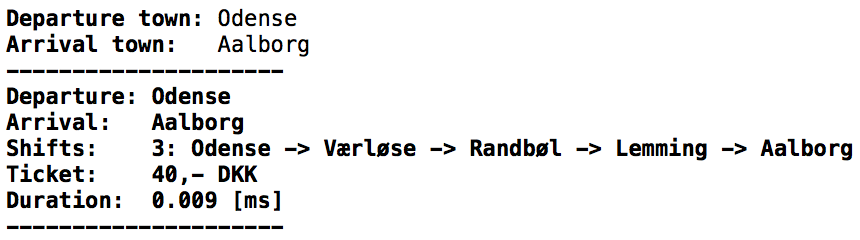
\includegraphics[width=0.7\textwidth]{./graphics/ex1}
\caption{Output from editor: Odense to Aalborg.}
\label{fig:odense_Aalborg}
\end{figure}

	
\subsection{Odense to Holstebro}

\begin{figure}[th!]
\centering
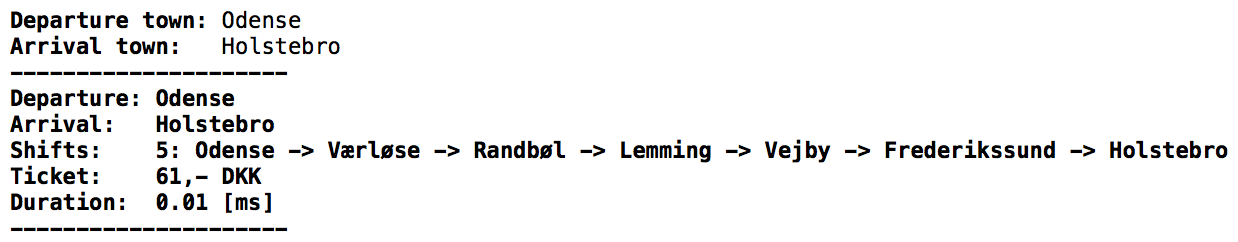
\includegraphics[width=0.7\textwidth]{./graphics/ex2}
\caption{Output from editor: Odense to Holstebro.}
\label{fig:odense_holstebro}
\end{figure}

\subsection{Odense to Humlebæk}


\begin{lstlisting}[frame=single]
Departure: Odense\\
%Arrival:   Humlebæk\\
%Shifts:    6: Odense -> Værløse -> Randbøl -> Lemming -> Gram -> Øster Vrå -> Humlebæk\\
Ticket:    62,- DKK\\
Duration:  68.65 [ms]\\
---------------------
\end{lstlisting}

\begin{figure}[th!]
\centering
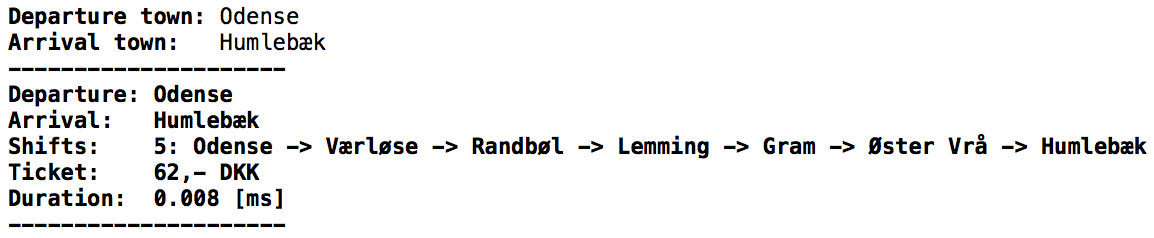
\includegraphics[width=0.7\textwidth]{./graphics/ex3}
\caption{Output from editor: Odense to Humlebæk.}
\label{fig:odense_humlebæk}
\end{figure}






